\documentclass[border=4pt]{standalone}

\usepackage[T1]{fontenc}
\usepackage[utf8]{inputenc}
\usepackage{amsmath}
\usepackage{xcolor}
\usepackage{tikz}
\usetikzlibrary{positioning, fit, calc, arrows.meta, backgrounds}

\begin{document}
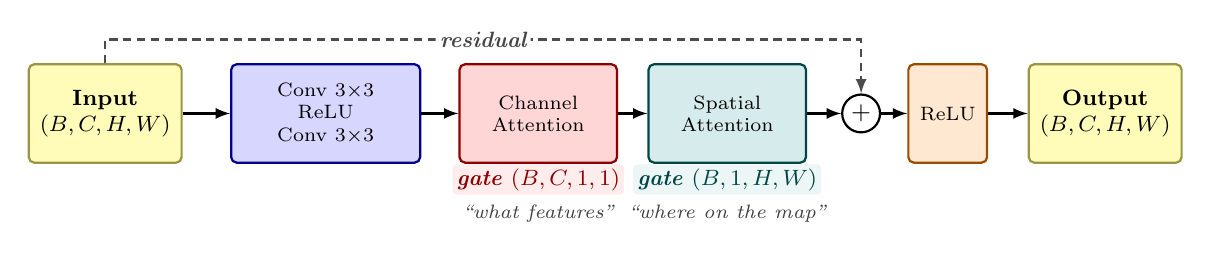
\begin{tikzpicture}[
    >=latex,
    blk/.style={draw, rounded corners=2pt, align=center, thick, inner sep=4pt, font=\scriptsize},
    conv/.style={blk, fill=blue!16, draw=blue!55!black, minimum width=2.4cm, minimum height=1.25cm},
    chann/.style={blk, fill=red!16, draw=red!55!black, minimum width=2.0cm, minimum height=1.25cm},
    spat/.style={blk, fill=teal!16, draw=teal!55!black, minimum width=2.0cm, minimum height=1.25cm},
    actrelu/.style={blk, fill=orange!18, draw=orange!60!black, minimum width=1.0cm, minimum height=1.25cm},
    io/.style={blk, fill=yellow!28, draw=yellow!55!black, minimum width=1.7cm, minimum height=1.25cm, font=\footnotesize\bfseries},
    op/.style={draw, circle, thick, inner sep=1.5pt, font=\small},
    flow/.style={->, thick},
    resid/.style={->, thick, densely dashed, gray!60!black},
    sublbl/.style={font=\scriptsize\itshape, text=gray!50!black, fill=white, inner sep=1.5pt},
    grouplbl/.style={font=\footnotesize\bfseries\itshape, rounded corners=1.5pt, inner sep=1.5pt, fill=white},
]

\node[io]      at (0,    0) (in)   {Input\\$(B,C,H,W)$};
\node[conv]    at (2.8,  0) (c1)   {Conv $3{\times}3$\\ReLU\\Conv $3{\times}3$};
\node[chann]   at (5.5,  0) (ca)   {Channel\\Attention};
\node[spat]    at (7.9,  0) (sa)   {Spatial\\Attention};
\node[op]      at (9.6,  0) (sum)  {$+$};
\node[actrelu] at (10.7, 0) (relu) {ReLU};
\node[io]      at (12.7, 0) (out)  {Output\\$(B,C,H,W)$};

\foreach \a/\b in {in/c1, c1/ca, ca/sa, sa/sum, sum/relu, relu/out}
    \draw[flow] (\a) -- (\b);

\coordinate (residL) at ($(in.north) + (0, 0.30)$);
\coordinate (residR) at (residL -| sum.north);
\draw[resid] (in.north) -- (residL) -- (residR) -- (sum.north);
\node[grouplbl, text=gray!55!black, fill=white] at ($(residL)!0.5!(residR)$) {residual};

\node[grouplbl, text=red!55!black,  fill=red!7]  (cagate) at ([yshift=-0.20cm]ca.south) {gate $(B,C,1,1)$};
\node[grouplbl, text=teal!55!black, fill=teal!7] (sagate) at ([yshift=-0.20cm]sa.south) {gate $(B,1,H,W)$};

\node[sublbl, anchor=north] at ([yshift=-0.06cm]cagate.south) {``what features''};
\node[sublbl, anchor=north] at ([yshift=-0.06cm]sagate.south) {``where on the map''};

\end{tikzpicture}
\end{document}
